\chapter{Ecosystems: Chemical and Information Networks}

\begin{kaichang}
Next time you pass a pond, scoop up a cup of water in an ordinary glass. Hold it against the light. You will probably see a faint green tinge and a few drifting specks almost too small to make out. A little black mud may settle at the bottom, smelling slightly fishy.

Now guess: how many ``residents'' live in this apparently quiet water? Ten? A hundred? And where are the leaves that fell into the pond last autumn? Are they still in the pond, or have they ``disappeared''?

Write both answers down. In this penultimate chapter, we will bring everything collected over the previous eighty-five chapters---atoms, chemical bonds, energy, enzymes, DNA, and evolution---to this pond and see what drama they perform together on a planetary scale.
\end{kaichang}

\textbf{Translator safety note:} Observe from a safe bank with adult supervision; do not enter the water, taste it, or deliberately sniff samples. Avoid water with scum, discoloration, or an unusual smell, which may indicate a harmful bloom. Use a dedicated, clearly marked observation container and wash hands after handling it. See \href{https://cdc.gov/harmful-algal-blooms/prevention/index.html}{CDC harmful-algal-bloom precautions} and \href{https://www.cdc.gov/healthy-pets/about/fish.html}{CDC aquarium-water hygiene guidance}.

\section{The Leaves Have Not Disappeared}

Start with the visible world. Thick layers of fallen leaves accumulate in the park in autumn, yet little remains by the following spring. After the snow melts, part the grass and you find only unrecognizable brown fragments. Where did the leaves go?

The usual answer is ``They rotted'' or ``They're gone.'' But look through the lens you acquired in Chapter 1: matter consists of atoms, and atoms cannot simply disappear, except in nuclear reactions, which are not happening here. The carbon, hydrogen, oxygen, nitrogen, and phosphorus atoms in a leaf must be somewhere now. Find them, and you have found the entrance to an ecosystem.

The truth is that the leaves were \emph{eaten}, bit by bit, by bacteria, fungi, springtails, and earthworms in the soil. Enzymes in these decomposers' cells (Chapter 49) break apart leaf cellulose and proteins, then cellular respiration (Chapter 53) oxidizes the carbon skeletons step by step. Some leaf carbon becomes carbon dioxide, \chem{CO_2}, breathed back into the air; some becomes protein in decomposers' bodies; some remains as soil humus. Nitrogen becomes ammonium salts and nitrates, is absorbed by nearby grass roots, and grows into new leaves next year.

Not one atom is missing, and not one has been added. The leaf has not disappeared; it has merely \emph{changed its arrangement} and moved house.

Zoom out and a web appears: grass is eaten by grasshoppers, grasshoppers by frogs, and frogs by snakes. When the snakes, frogs, grasshoppers, and grass die, decomposers receive them all. This is a \textbf{food web}, not a straight ``chain,'' because almost every organism has more than one food and more than one enemy. A food web is an ecosystem's ``matter-flow diagram'': whose body will receive the atoms from whose body next?

\section{One-Way Streets and Roundabouts}

Two completely different things flow through a food web, obeying very different rules. Separating them is the key to understanding the whole ecosystem.

The first is \textbf{energy}. It almost always enters through the same doorway: sunlight. Producers---plants, algae, and cyanobacteria---use photosynthesis to convert light energy into chemical energy stored in organic molecules such as glucose. See Chapter 54 for details, and remember that the released oxygen comes from water, not carbon dioxide. Energy then passes from level to level through the food web. Each transfer pays a heavy ``tax'': cellular respiration converts much of the chemical energy into heat that dissipates into the surroundings. Once dispersed, that heat cannot be recovered to become glucose again. Energy therefore follows a \textbf{one-way street} through an ecosystem: sunlight in, heat out, with no return journey. Earth's ecosystem keeps running because the Sun never shuts off its energy supply, with a little help from Earth's residual internal heat.

The second is \textbf{matter}: atoms of carbon, nitrogen, phosphorus, sulfur, and other elements. They travel around a \textbf{roundabout}, entering organisms from air, water, and soil, changing hands through the food web, and eventually being dismantled by decomposers and picked up by producers for another circuit. Earth receives almost only energy from the Sun, scarcely any matter; annual meteor dust is negligible compared with the biosphere. Ecosystems must therefore carefully \emph{recycle} every atom.

\begin{wuqu}
``Energy is recycled through the food chain.'' This widespread statement confuses energy with matter. The test is simple: if energy truly cycled, a completely sealed ecological bottle without light should run forever. In fact, once placed in a dark cupboard, all its residents die within days or weeks. Photosynthesis stops, no new energy enters, and the chemical energy stored in organisms soon leaks away as heat. There is the counterexample: matter can circulate in a sealed bottle for a long time, but energy needs a continuous external supply. Your desk lamp, an aquarium heater, and the Sun above the whole biosphere illustrate the same principle: \textbf{matter needs recycling; energy needs replenishment}.
\end{wuqu}

\begin{qiaoliang}
How much ``tax'' does each energy transfer pay? Measurements of real lakes, grasslands, and forests show that, on average, only approximately $10\%$ of the energy at one level is ``deposited'' in bodies at the next. The rest becomes respiratory heat or leaves as undigested food waste. This is a rough figure---different systems range from $5\%$ to $20\%$---but a powerful tool for estimation.

Suppose a grassland fixes $10000$ units of chemical energy through photosynthesis in a year. Grass-eating insects retain approximately $10\%\times 10000=1000$ units; insect-eating birds, approximately $100$ units; and raptors eating those birds, approximately $10$ units. In other words, \textbf{every 1 unit of energy at the top of the food web requires approximately 1,000 units at the bottom}. This directly explains the scarcity of top predators: a grassland can support tens of millions of grasses, a million insects, and thousands of birds, but only a few hawks. It also explains why eating grain uses less land than eating meat. Growing grain to feed pigs and then eating pork adds another step up the energy ladder, sharply reducing the output from the same land. This ecological rule of thumb, the ``ten-percent rule,'' comes not from ecological magic but from the thermodynamics of Chapters 27 and 53: each energy conversion incurs losses, and dissipated heat cannot be reclaimed.
\end{qiaoliang}

Here are both rules in one diagram. This is a human-made representation; box sizes and arrow thicknesses are merely schematic:

\begin{center}
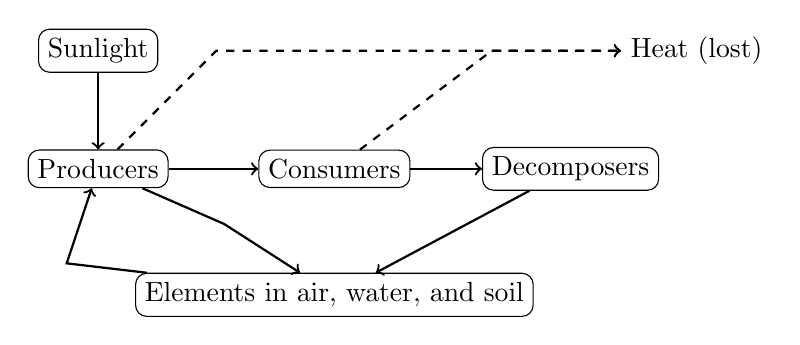
\begin{tikzpicture}[scale=1.0]
\node[draw, rounded corners] (sun) at (0,2.4) {Sunlight};
\node[draw, rounded corners] (prod) at (0,0.9) {Producers};
\node[draw, rounded corners] (cons) at (3,0.9) {Consumers};
\node[draw, rounded corners] (deco) at (6,0.9) {Decomposers};
\node[draw, rounded corners] (pool) at (3,-0.7) {Elements in air, water, and soil};
\node (heat) at (7.6,2.4) {Heat (lost)};
\draw[->, thick] (sun) -- (prod);
\draw[->, thick] (prod) -- (cons);
\draw[->, thick] (cons) -- (deco);
\draw[->, thick] (prod) -- (1.6,0.2) -- (pool);
\draw[->, thick] (deco) -- (pool);
\draw[->, thick] (pool) -- (-0.4,-0.3) -- (prod);
\draw[->, thick, dashed] (prod) -- (1.5,2.4) -- (heat);
\draw[->, thick, dashed] (cons) -- (5,2.4) -- (heat);
\end{tikzpicture}
\end{center}

Atoms flow along the solid arrows---notice the loop back to producers---while dashed arrows show energy leaking away at successive levels. The diagram captures the chapter's theme: an ecosystem is a machine driven by energy flow and maintained by matter cycling.

\section{Three Cycles and Invisible Engineers}

There is not just one roundabout but several parallel routes, one for each element. We will choose three especially important to life: carbon, nitrogen, and phosphorus.

The \textbf{carbon cycle} is the most familiar. Atmospheric \chem{CO_2} is fixed into organic matter through photosynthesis, passes through the food web, and returns to the atmosphere through respiration and decomposition. Some carbon takes a ``slow lane'': it sinks to the seafloor and becomes limestone, or is buried underground and becomes coal and oil, locked away for millions of years until volcanic eruptions or human extraction return it to the atmosphere. A chemical equilibrium guards the carbon cycle's atmospheric entrance and exit:

\[\chem{CO_2} + \chem{H_2O} \rightleftharpoons \chem{H^+} + \chem{HCO_3^-}\]

The more \chem{CO_2} the ocean absorbs, the farther the equilibrium shifts right and the more acidic seawater becomes. As we will see, this compact reaction equation affects the fate of the entire planet.

The main actors in the \textbf{nitrogen cycle} are neither plants nor animals but microbes. Air is $78\%$ nitrogen gas, \chem{N_2}, yet the triple bond between its two atoms is exceptionally strong (Chapter 21), beyond plants' ability to ``chew.'' Only nitrogen-fixing bacteria, such as the rhizobia in legume root nodules, can split \chem{N_2}. Their nitrogenase accomplishes at ordinary temperature and pressure what humans need high temperatures and pressures to achieve in the industrial Haber process (Chapter 44). Once the ammonia, \chem{NH_3}, produced by fixation becomes ammonium, \chem{NH_4^+}, nitrifying bacteria oxidize it step by step into nitrate, \chem{NO_3^-}:

\[\chem{NH_4^+} \rightarrow \chem{NO_2^-} \rightarrow \chem{NO_3^-}\]

Plants absorb nitrate to make proteins and DNA; animals eat plants; decomposers break excrement and dead bodies back into ammonium. Finally, denitrifying bacteria in oxygen-poor soil convert nitrate back into \chem{N_2}, returning it to the atmosphere and closing the loop. The nitrogen in every breath you take may just have completed a journey through bacteria and legumes.

The \textbf{phosphorus cycle} has one crucial difference: no ``air route.'' Phosphorus has almost no stable gaseous compounds. It must enter soil and water through rock weathering, be used by organisms, and finally sink with sediments to the seafloor, returning only after immense spans of time when crustal uplift exposes it to weathering again. Of the three cycles, it is therefore the slowest and most prone to ``supply interruptions.'' In many fields and lakes, phosphorus is precisely the limiting factor for biological growth.


Compare the three cycles:

\begin{table}[h]
\centering
\begin{tabular}{llll}
\toprule
Cycle & Main reservoirs & \shortstack[l]{Entry into the\\biosphere} & \shortstack[l]{Key microbial\\roles} \\
\midrule
Carbon & \shortstack[l]{Air, oceans,\\rocks} & \shortstack[l]{Photosynthesis\\fixes \chem{CO_2}} & \shortstack[l]{Decomposers\\release \chem{CO_2}} \\
Nitrogen & Air (\chem{N_2}) & \shortstack[l]{Fixation breaks\\the triple bond} & \shortstack[l]{Fixing, nitrifying,\\denitrifying bacteria} \\
Phosphorus & \shortstack[l]{Rocks,\\sediments} & \shortstack[l]{Rock weathering\\(very slow)} & \shortstack[l]{Decomposers recycle\\from dead organisms} \\
\bottomrule
\end{tabular}
\end{table}

Notice the implication: \textbf{without microbes, the cycles break}. If bacteria and fungi all vanished tomorrow, leaves and dead bodies would pile up, nitrogen would be locked in organic matter, plants would lack nitrogen and phosphorus, and food webs would collapse from the bottom. Chapter 62 explained that your own body is an ecosystem involving microbes. Here is the enlarged version: the whole biosphere likewise depends on these invisible ``plumbers.''

\section{Information: The Network's Third Flow}

Besides energy and matter, a third thing flows through food webs: \textbf{information}, and it too is chemical.

When aphids chew a bean seedling, the plant releases particular volatile molecules into the air. Neighboring bean seedlings ``smell'' them and activate defense genes in advance, producing substances the aphids find difficult to swallow. Caterpillar-damaged corn releases signals attracting the caterpillars' enemies, parasitoid wasps---effectively ``calling the police.'' Fungal threads connect multiple trees underground, allowing sugars, nitrogen, and warning signals to travel through a ``wood-wide web''; see Chapter 61's discussion of boundaries for details and debate. Fireflies flash mating codes using the luciferin--luciferase reaction, the chemiluminescence mentioned in Chapter 53. Ants write chemical signposts to food on the ground with pheromones.

These signals are carried by molecules encountered repeatedly in this book: terpenes, esters, and peptides. Receptor proteins receive them, applying the same principles as the cellular signaling in Chapter 58, but expanded from a cell membrane to a whole forest. Molecules are emitted, diffuse, are captured by receptors, and trigger behavioral changes: that is information flow. The ecosystem's web is both chemical, involving matter and energy, and informational, involving signals and responses.

\begin{shiyan}
\textbf{Build a sealed ecological bottle to observe ``matter recycling and energy replenishment.''}

\textbf{Translator safety note:} Do not follow the sealed-snail or dark-cupboard animal treatment below: it deliberately risks oxygen deprivation and death. Omit animals and ask a teacher to assess a plant-only observation or use published observations. Do not release purchased plants, snails, or experimental water into any pond, including the collection site; consult local wildlife authorities about safe disposal or rehoming. Follow \href{https://www.cdc.gov/healthy-pets/about/fish.html}{CDC water-handling hygiene} and \href{https://www.fws.gov/learn/protect-your-waters}{USFWS aquatic-species precautions}. This caution supplements, rather than replaces, the translated source protocol.

Materials: a clear glass jar with a sealing lid, approximately 1--2 liters; washed fine sand or small stones; a cup of pond or river water; several aquatic plant sprigs, such as hornwort or centipede grass, sold in flower-and-bird markets or aquarium shops; and optionally one or two apple snails.

Procedure: (1) Cover the bottom with a 2-centimeter layer of stones. (2) Add pond water until the jar is four-fifths full. (3) Add plants and snails. (4) Seal the lid and place the jar on a \emph{bright windowsill out of direct sunlight}, which would overheat it. (5) Label it with the date and observe weekly for at least a month.

What to observe: do the plants grow new leaves? Are the snails alive and grazing the green film on the glass? Does this film of algae increase or decrease over time? Put an identically prepared second bottle in a dark cupboard as a control and compare the two weekly.

Safety: use only pond water and aquatic plants; add no chemicals other than tap water. Wash your hands after opening the jar to observe it, and do not drink its water. At the end, return plants and snails to their source pond or dispose of them appropriately, not into drains or unfamiliar waters, to avoid spreading species.

The principle: a sealed jar admits light but no matter. Plants photosynthesize, producing organic matter and oxygen; snails eat algae and consume oxygen through respiration. Microbes decompose snail waste, releasing \chem{CO_2}, nitrogen, and phosphorus for the plants to reuse. Matter circles inside the jar, while sunlight outside the window replenishes energy. The dark control bottle shows how long this little machine lasts after its energy input is cut off.
\end{shiyan}

\section{Diversity: The Network's Redundancy}

If your ecological bottle contains only one aquatic plant species, its death can collapse the bottle. If plants, algae, snails, and microbes each perform their roles, other members can partly compensate when one encounters trouble. This illustrates an ecological rule repeatedly tested and refined: \textbf{ecosystems richer in species often withstand disturbance better}.

Engineering intuition helps explain why. A building supported by one column collapses if it breaks. With several columns, the others can share the load when one fails. Engineers call this ``redundancy.'' Multiple species with similar functions---several carbon-fixing plants or several pollinating insects---give an ecosystem redundancy. ``Biodiversity'' may sound like a slogan, but unpacked it is a property of network topology: more nodes and denser connections make a single point of failure less fatal.

Do not push this to an extreme. More diversity is not always better regardless of species: rampant nonnative species can dismantle local networks, as water hyacinths choke waterways. Losing keystone species, such as pollinators or top predators, can matter far more than losing an equal number of ordinary species. Diversity buys a \emph{buffer against change}, not insurance against every failure.

Biodiversity also provides a whole package of ``ecosystem services'': plants and microbes purify water and form soil; insects pollinate crops, with approximately one-third of the world's food crops depending on animal pollination; wetlands reduce flooding; forests fix carbon dioxide. Replacing these services artificially with water-treatment plants, hand pollination, or embankments would cost astronomical sums. Fruit growers in Sichuan already hire people to pollinate pear blossoms individually with brushes because local bees are insufficient. That is what replacing an interrupted service looks like: expensive and slow.

\begin{zhengju}
How do scientists know that matter cycles within ecosystems and that people can alter those cycles? Some of the most direct evidence came from a bold experiment: ``take apart'' an entire forest and see.

Beginning in 1963, American ecologists Bormann and Likens developed a classic experiment at Hubbard Brook Experimental Forest in New Hampshire. They selected neighboring small watersheds, each comprising a hillside and its stream, and spent several years measuring the ``budget'': how much calcium, potassium, and nitrate entered in rain and left in streamwater. In healthy forest, most nutrient outputs proved far smaller than inputs. The forest \emph{retained} nutrients within itself, cycling them tightly.

Then came the decisive step. In the winter of 1965, they cut every tree in one watershed and used herbicides to suppress regrowth, leaving the other watersheds as controls. Stream nitrate concentrations soared to dozens of times their pre-cutting levels, and calcium and potassium were also lost in large quantities. Removing vegetation opened a valve in nutrient cycling: soil nitrifying bacteria kept producing nitrate, but there were no roots to absorb it, so rain washed the nutrients away. Control watersheds showed no corresponding change, excluding alternatives such as unusual rainfall that year.

This meant more than ``Cutting trees is bad.'' For the first time, a measurable, controlled approach demonstrated that \textbf{nutrient cycling is a property of the ecosystem as a whole}, maintained jointly by plants, soil, and microbes; remove any link and the cycle leaks. Later long-term monitoring in the same forest documented acid-rain effects and decades of slow recovery, becoming a benchmark for long-term ecological experiments. Notice the methodological character: not intuitive assertion, but a baseline, controls, one changed variable, and data allowed to speak.
\end{zhengju}

\section{When the Network Is Stretched}

Understanding the ``one-way street plus roundabout'' helps make sense of today's ecological news: nearly all these problems involve human activity putting strain on those two rules.

\textbf{Eutrophication}: nitrogen and phosphorus fertilizers wash from fields into lakes, effectively air-dropping rations to algae. Algae proliferate in blooms, then die and are decomposed by bacteria, which consume large amounts of oxygen and suffocate fish and other organisms. A cyanobacterial bloom in Lake Taihu in 2007 made tap water foul-smelling for millions in Wuxi because nitrogen and phosphorus inputs exceeded the lake's cycling capacity. Natural cycling had not ``malfunctioned''; excess inputs had \emph{overloaded} it, like traffic far beyond a roundabout's design capacity.

\textbf{Ocean acidification}: the short equilibrium equation above is shifting on a global scale. Burning fossil fuels has raised atmospheric \chem{CO_2} from approximately $280\ \mathrm{ppm}$ before the Industrial Revolution to over $420\ \mathrm{ppm}$ today. The ocean has absorbed approximately a quarter of it, lowering seawater pH. Acidification itself is not immediately lethal to many organisms; the serious difficulty comes downstream. Carbonate, \chem{CO_3^{2-}}, declines, making calcium-carbonate shells harder for corals and shellfish to build---a planetary version of Chapter 39's precipitation equilibria. Push one equilibrium, and the chain of life depending on it must adjust.

\textbf{Pollutant biomagnification}: this is the dark side of the ten-percent rule. Some substances, such as mercury and persistent organic pollutants, are \emph{not readily} dismantled by decomposers after entering food webs. Energy shrinks approximately tenfold per level, yet organisms largely retain these substances from their food. Concentrations consequently rise step by step: negligible in plankton, higher in small fish, higher still in large fish, and potentially amplified tens of thousands of times in raptors, large fish, and humans at the top. This is how DDT thinned top predators' eggshells and caused reproductive failure in the last century. A pollutant's danger depends not only on acute toxicity but also on whether it can leave the food web.

\textbf{Climate change}: in two centuries, humans have forcibly merged the carbon cycle's slow lane---coal, oil, and limestone---into its fast lane. Extra \chem{CO_2} strengthens the greenhouse effect (Chapter 38), forcing Earth's ecosystem to find a new balance in its energy budget. The biosphere's chemical and information networks, from pollination timing to ocean currents, must all change with it.

Together these four issues share a picture: \textbf{human activities have changed no chemical law, only the magnitudes of flows}---nitrogen, phosphorus, carbon, and energy flows. Their relative balance is precisely what maintains the ecosystem's network.

\section{The Model's Boundaries}

When is this chapter's model useful, and when does it demand caution?

``One-way energy, cycling matter'' is highly reliable at large scales, but Earth is not absolutely closed. Meteorites bring in some matter, hydrogen and helium escape the upper atmosphere each year, and human spacecraft carry terrestrial atoms permanently beyond the biosphere. The ten-percent rule is a rough average; a particular food chain can differ severalfold, so exact calculations with it will be wrong. Box-and-arrow diagrams reduce rivers, lakes, and oceans to a few ``reservoirs,'' each of which is actually internally uneven and changing. As for ``diversity causes stability,'' evidence is good in controlled small-scale experiments, but the relationship becomes more complicated across entire landscapes. This remains an open question for Chapter 87.

\section{Back to That Cup of Water}

Look again at the opening cup of pond water. Among the backlit specks are single-celled algae converting photons into chemical bonds. In the foul black mud, denitrifying bacteria gradually turn nitrate back into nitrogen under oxygen-poor conditions. The barely visible green film on the glass is a microbial ``city'' whose residents coordinate through chemical signals. Left in sunlight, a still cup of pond water can maintain itself for a long time because it is a miniature planet: energy enters through the window and leaves as heat; carbon, nitrogen, and phosphorus cycle inside; information passes among molecules.

The fallen leaves did not disappear. They were dismantled, passed along, and reassembled, and now continue as carbon dioxide, new leaves, and bacterial bodies. Was your guess right?

This book began with a question: why does matter change in these ways? We started with atoms, passed through bonds, reactions, and energy, and entered cells, DNA, and evolution. Now, looking back from the scale of the whole biosphere, we see the same uninterrupted causal chain: every act of photosynthesis and decomposition in pond water obeys Chapter 27's energy bookkeeping; nitrogen-fixing enzymes are relatives of Chapter 49's proteins; the signals connecting forests follow Chapter 58's receptor principles; and this network changes over immense spans of time through the evolution discussed in Part X. \textbf{At planetary scale, there is no new chemistry, only chemistry on a new scale.}

Scale itself, however, brings new mysteries. How far can we predict and manage such a network? In the next and final chapter, we will visit questions science cannot yet answer. That is the book's true ending: not ``We know everything,'' but ``Here is how far our knowledge reaches.''

\begin{tiaozhan}
Try estimating photosynthesis's share using planetary numbers. Average solar power arriving at the top of Earth's atmosphere is approximately $340$ watts per square meter, accounting for the planet's spherical shape and the fact that half the time is night. Earth's surface area is approximately $5.1\times 10^{14}$ square meters, giving total incoming solar power of approximately $1.7\times 10^{17}$ watts. Measured global photosynthesis fixes approximately $4\times 10^{21}$ joules of chemical energy each year. Dividing by the year's approximately $3.2\times 10^7$ seconds gives average power of approximately $1.2\times 10^{14}$ watts. Dividing the two shows that photosynthesis intercepts only approximately $0.07\%$ of the solar energy reaching Earth. This tiny fraction sustains the entire biosphere. Meanwhile, humanity's current total energy use, approximately $2\times 10^{13}$ watts, is already approximately one-sixth of global photosynthetic carbon fixation's power. The numbers are rough, but the orders of magnitude are real: our species' energy consumption is now comparable to the planet's entire ``production line.''
\end{tiaozhan}

\section*{Exercises}

\begin{sikaoti}
\item Draw a matter-flow diagram for a park in your city or a corner of your campus. Identify producers, consumers, and decomposers, draw three possible carbon-atom paths with arrows, and separately draw the full energy pathway from entry to departure using dashed lines. What fundamental difference is there between the shapes of the energy and matter pathways?
\item A sealed ecological bottle lasts months in sunlight but collapses within weeks in a dark cupboard. Using ``energy's one-way street and matter's roundabout,'' explain what cycles inside the bottle and what leaks away.
\item Suppose a herbicide kills only nitrifying bacteria without harming plants directly. Use the nitrogen cycle to predict what happens to the field after several months. Draw the changes in nitrogen-atom flows.
\item Mercury concentration in plankton is $1$ unit and increases approximately $10$-fold per trophic level. What concentrations would you expect in plankton-eating small fish, large fish eating them, and people eating the large fish? How does this explain stricter eating advice for large predatory fish than for small fish?
\item During a Lake Taihu cyanobacterial bloom, someone proposes raising more fish and shrimp to eat all the algae. Using energy-transfer efficiency and eutrophication's causes, explain why this generally fails as a stand-alone solution. Which ``valve'' really needs controlling?
\item Find a news story about biodiversity conservation and write three sentences using this chapter's redundancy and information-network perspectives. What function might this species or habitat perform? Which connections might its loss affect?
\end{sikaoti}
